% (c)~2014 Dimitrios Vrettos - d.vrettos@gmail.com
% (c)~2014 Claudio Carboncini - claudio.carboncini@gmail.com
% (c)~2015 Daniele Zambelli daniele.zambelli@gmail.com
% (c)~2015 Maria Antonietta Pollini

% (c) 2014 Daniele Zambelli - daniele.zambelli@gmail.com

\newcommand{\quadratopitagorico}[3]{%
  \coordinate (a) at (0, 0);
  \coordinate (b) at (#1, 0);
  \coordinate (c) at (#1, #1);
  \coordinate (d) at (0, #1);
% \colorlet{anglecolor}{green!50!black}

  \begin{scope}[line join=round, line cap=round]
    \draw[thick, Maroon!50!black] (a)--(b)
          node [black, sloped, midway, below] {#2} -- (c) -- cycle 
          node [black, sloped, midway, above] {#3};
    \draw[thick, Maroon!50] (a)--(d)--(c);
%     \draw [->, anglecolor, thick](#1*.3, 0) arc(0:45:#1*.3);
    \draw [->, thick](#1*.3, 0) arc(0:45:#1*.3);
%     \draw (#1*.45, #1*.15) node [anglecolor] {$45 \text{°}$};
    \draw (#1*.45, #1*.15) node {$45 \text{°}$};
  \end{scope}
}


\newcommand{\triequipitagorico}[1]{%
  \coordinate (a) at (0, 0);
  \coordinate (m) at (#1/2, 0);
  \coordinate (b) at (#1, 0);
  \coordinate (c) at (#1/2, #1 * 0.8660254);

  \begin{scope}[line join=round, line cap=round]
    \draw[thick, Maroon!50!black] (a)--
          (m)
          node [black, sloped, midway, below] {$\frac{l}{2}$} -- 
          (c)
          node [black, sloped, midway, above, xshift=-10pt] 
               {$l \cdot \frac{\sqrt{3}}{2}$} -- 
          cycle 
          node [black, midway, above left] {$l$};
    \draw[thick, Maroon!50] (m)--(b)--(c);
%     \draw [->, anglecolor, thick](#1*.3, 0) arc(0:60:#1*.3);
    \draw [->, thick](#1*.15, 0) arc(0:60:#1*.15);
%     \draw (#1*.45, #1*.15) node [anglecolor] {$60 \text{°}$};
    \draw (#1*.25, #1*.08) node  {$60 \text{°}$};
  \end{scope}
}


% \begin{figure}[h]
% \begin{minipage}{.40\textwidth}
% 
% \end{minipage}
% \begin{minipage}{.60\textwidth}
% \begin{inaccessibleblock}[?]
% \centering
%   \input{\folder lbr/?.pgf}
%   \caption{?.} \label{fig:?_?}
% \end{inaccessibleblock}
% \end{minipage}
% \end{figure}

% \begin{wrapfloat}{figure}{r}{0pt}
% \includegraphics[scale=0.35]{img/?.png}
% \caption{?}
% \label{fig:?_?}
% \end{wrapfloat}
% 
% \begin{center} \input{\folder lbr/?.pgf} \end{center}

\begin{comment}

\begin{inaccessibleblock}[]
\begin{center}
  \
\end{center}
\end{inaccessibleblock}
\end{comment}

\begin{comment}
 
 \begin{minipage}{.45\textwidth}
  
 \end{minipage}
 \begin{minipage}{.25\textwidth}
  
 \end{minipage}
 \begin{minipage}{.3\textwidth}
  
 \end{minipage}
 
\end{comment}

\chapter{Disequazioni}

\section{Risoluzione delle disequazioni di secondo grado}
\label{sec:diseq_secondo_grado}

Una disequazione di secondo grado si presenta in una delle seguenti forme:
\[ax^2+bx+c<0;\quad ax^2+bx+c\le 0;\quad ax^2+bx+c\ge0;\quad ax^2+bx+c> 0\]

Ricordiamo che risolvere una disequazione in un'incognita significa 
determinare l'insieme dei valori da attribuire all'incognita affinché la 
disequazione sia verificata.
Come per le disequazioni di primo grado anche per quelle di secondo grado
dobbiamo studiare il segno del trinomio e poi individuare l'insieme soluzione.

\subsection{Studio del segno di un trinomio di secondo grado}
\label{sec:diseq_trinomio}

Per studiare il segno di un polinomio di secondo grado seguiamo un 
procedimento in due passi:

\begin{enumerate}
 \item Equazione associata
Risolvendo l'equazione associata al polinomio troviamo gli zeri della 
funzione cioè i punti in cui il grafico della funzione incontra l'asse~x. 

A seconda del valore del discriminante l'equazione può avere 
nessuna soluzione reale (\(\Delta<0\)), 
soluzioni reali coincidenti (\(\Delta=0\)), 
soluzioni reali distinte (\(\Delta>0\)).

 \item Grafico della funzione associata
Disegnando il grafico della funzione associata al polinomio si individuano 
gli intervalli in cui il polinomio è positivo, il grafico è sopra l'asse~x 
o negativo, il grafico è sotto l'asse~x.

Se il coefficiente del termine di secondo grado è minore di zero (\(a<0\)) 
la parabola ha la concavità rivolta verso il basso, se è maggiore di zero 
(\(a>0\)) la parabola ha la concavità rivolta verso l'alto. 
\end{enumerate}

% \begin{exrig}
\begin{esempio}
Studiare i segno del polinomio: \(x^2-2x-3\)

\begin{enumerate}
 \item
  Equazione Associata:~\(x^2-2x-3=0 \sRarrow 
                        \left(x-3 \right)\left(x+1\right)=0 \sRarrow 
                        x_1=-1~\cup~x_2=+3\)
 \item 
  \begin{minipage}{.45\textwidth}
  Funzione Associata: \(y = x^2-2x-3 \quad \rightarrow\)
  \end{minipage}
  \begin{minipage}{.30\textwidth}
  \parabolaamadma{-1}{3}
  \end{minipage}
\end{enumerate}

\end{esempio}

Una volta studiato il segno del polinomio, risolvere una disequazione nella 
forma \(f(x) \lessgtr 0\) consiste nell'aggiungere un ulteriore passo 
piuttosto banale: individuare l'insieme soluzione.

\begin{esempio}
Risolvi le seguente disequazioni utilizzando lo studio del segno del trinomio 
di secondo grado.

%%%%%%%%%%%%%%%%%%%%%% Usare lo schema già utilizzato per il primo grado


\begin{comment}
\begin{minipage}{.49\linewidth}
 
\end{minipage}
\hfill
\begin{minipage}{.49\linewidth}
 
\end{minipage}
\end{comment}

\begin{itemize}
\item $x^2+x-2>0$.

\begin{enumerate}
 \item
  Equazione Associata:~\(x^2+x-2=0 \sRarrow 
                        \left(x-1 \right)\left(x+2\right)=0 \sRarrow 
                        x_1=-2~\cup~x_2=+1\)
 \item 
  \begin{minipage}{.45\textwidth}
  Funzione Associata: \(y = x^2+x-2 \quad \rightarrow\)
  \end{minipage}
  \begin{minipage}{.30\textwidth}
  \parabolaamadma{-2}{+1}
  \end{minipage}
 \item 
 Insieme soluzione\\
 
  \begin{minipage}{.32\textwidth}
  Forma grafica\\[-.7em]
  
 \begin{center}
  \inteaa{8}{-2}{+1}
  \vspace{.4em}
 \end{center}
  \end{minipage}
  \begin{minipage}{.32\textwidth}
  Espressione con i predicati\\[-.3em]
  
 \begin{center}
  \(x<-2 \sor x>+1\)
  \vspace{1em}
 \end{center}
  \end{minipage}
  \begin{minipage}{.32\textwidth}
  Espressione con le parentesi\\[-.3em]
  
 \begin{center}
  \(\intervaa{-\infty}{-2}~\cup~\intervaa{1}{-\infty}\)
  \vspace{.8em}
 \end{center}
  \end{minipage}
\end{enumerate}

\item $x^2-4x+4\le0$.

\begin{enumerate}
 \item
  Equazione Associata:~\(x^2-4x+4=0 \sRarrow 
                        \left(x-2 \right)^2=0 \sRarrow 
                        x_{1,2}=+2\)
 \item 
  \begin{minipage}{.45\textwidth}
  Funzione Associata: \(y = x^2-4x+4 \quad \rightarrow\)
  \end{minipage}
  \begin{minipage}{.30\textwidth}
  \parabolaamadz{+2}
  \end{minipage}
 \item 
 Insieme soluzione\\
 
  \begin{minipage}{.32\textwidth}
  Forma grafica\\[-.7em]
  
 \begin{center}
  \puntoc{8}{+2}
  \vspace{.4em}
 \end{center}
  \end{minipage}
  \begin{minipage}{.32\textwidth}
  Espressione con i predicati\\[-.3em]
  
 \begin{center}
  \(x=2\)
  \vspace{1em}
 \end{center}
  \end{minipage}
  \begin{minipage}{.32\textwidth}
  Espressione con le parentesi\\[-.3em]
  
 \begin{center}
  \(\lbrace +2 \rbrace\)
  \vspace{.8em}
 \end{center}
  \end{minipage}
\end{enumerate}

\item $-x^2+2x-7>0$.

\begin{enumerate}
 \item
  Equazione Associata:~\(-x^2+2x-7=0 \sRarrow 
                        \dfrac{\Delta}{4} = -6 \sRarrow 
                        \text{N.H.S.R.}\)
 \item 
  \begin{minipage}{.45\textwidth}
  Funzione Associata: \(y = -x^2+2x-7 \quad \rightarrow\)
  \end{minipage}
  \begin{minipage}{.30\textwidth}
  \parabolaamidmi
  \end{minipage}
 \item 
 Insieme soluzione\\
 
  \begin{minipage}{.32\textwidth}
  Forma grafica\\[-.7em]
  
 \begin{center}
  \intv{8}
  \vspace{.4em}
 \end{center}
  \end{minipage}
  \begin{minipage}{.32\textwidth}
  Espressione con i predicati\\[-.3em]
  
 \begin{center}
  \(\nexists x \in \R\)
  \vspace{1em}
 \end{center}
  \end{minipage}
  \begin{minipage}{.32\textwidth}
  Espressione con le parentesi\\[-.3em]
  
 \begin{center}
  \(\emptyset\)
  \vspace{.8em}
 \end{center}
  \end{minipage}
\end{enumerate}

\item \(2x^2-5 \le 0\).

\begin{enumerate}
 \item
  Equazione Associata:~\(2x^2-5=0 \sRarrow 
                        x_{1, 2}= \mp \sqrt{\dfrac{5}{2}}\)
 \item 
  \begin{minipage}{.45\textwidth}
  Funzione Associata: \(y = 2x^2-5 \quad \rightarrow\)
  \end{minipage}
  \begin{minipage}{.30\textwidth}
  \parabolaamadma{-\sqrt{\dfrac{5}{2}}}{+\sqrt{\dfrac{5}{2}}}
  \end{minipage}
 \item 
 Insieme soluzione\\
 
  \begin{minipage}{.32\textwidth}
  Forma grafica\\[-.7em]
  
 \begin{center}
  \inticc{8}{-\sqrt{\dfrac{5}{2}}}{+\sqrt{\dfrac{5}{2}}}
  \vspace{.4em}
 \end{center}
  \end{minipage}
  \begin{minipage}{.32\textwidth}
  Espressione con i predicati\\[-.3em]
  
 \begin{center}
  \(-\sqrt{\dfrac{5}{2}} \le x \le +\sqrt{\dfrac{5}{2}}\)
  \vspace{1em}
 \end{center}
  \end{minipage}
  \begin{minipage}{.32\textwidth}
  Espressione con le parentesi\\[-.3em]
  
 \begin{center}
  \(\intervcc{-\sqrt{\dfrac{5}{2}}}{+\sqrt{\dfrac{5}{2}}}\)
  \vspace{.8em}
 \end{center}
  \end{minipage}
\end{enumerate}

\item \(-3x^2 + 2x > 0\).

\begin{enumerate}
 \item
  Equazione Associata:~\(-3x^2 + 2x=0 \sRarrow 
                        x_{1}= 0 \sand x_{2}= \dfrac{2}{3}\)
 \item 
  \begin{minipage}{.45\textwidth}
  Funzione Associata: \(y = -3x^2 + 2x \quad \rightarrow\)
  \end{minipage}
  \begin{minipage}{.30\textwidth}
  \parabolaamidma{0}{+\dfrac{2}{3}}
  \end{minipage}
 \item 
 Insieme soluzione\\
 
  \begin{minipage}{.32\textwidth}
  Forma grafica\\[-.7em]
  
 \begin{center}
  \intiaa{8}{0}{+\dfrac{2}{3}}
  \vspace{.4em}
 \end{center}
  \end{minipage}
  \begin{minipage}{.32\textwidth}
  Espressione con i predicati\\[-.3em]
  
 \begin{center}
  \(0 < x < +\dfrac{2}{3}\)
  \vspace{1em}
 \end{center}
  \end{minipage}
  \begin{minipage}{.32\textwidth}
  Espressione con le parentesi\\[-.3em]
  
 \begin{center}
  \(\intervaa{0}{+\dfrac{2}{3}}\)
  \vspace{.8em}
 \end{center}
  \end{minipage}
\end{enumerate}

\end{itemize}
\end{esempio}

% %%%%%%%%%%%%%%%%%%%%%%%%%%%%%%
% \section{Segno del trinomio a coefficienti letterali}
% Consideriamo il trinomio $t=kx^2+3x-7$ di secondo grado avente il primo 
% coefficiente dipendente dal parametro $k$. Come possiamo stabilire il segno 
% di 
% questo trinomio, al variare di $k$?
% Sappiamo che stabilire il segno di un trinomio significa determinare i valori 
% reali che attribuiti alla variabile indipendente $x$ rendono il trinomio 
% positivo, nullo o negativo. Evidentemente per valori reali diversi di $k$ 
% avremo 
% una diversa disequazione da risolvere; dobbiamo dunque cercare di analizzare 
% come varia il trinomio a seconda dei valori di $k$ e in seguito studiare il 
% segno del trinomio ottenuto. Questa analisi di situazioni diverse è la 
% \textit{discussione del trinomio a coefficienti parametrici}.
% 
% %%%%%%%%%%%%%%%%%%%%%%%%%%%%%%
% \conclusione Una disequazione di secondo grado si presenta sempre in una 
% delle 
% seguenti forme: ${ax}^2+{bx}+c>0$, ${ax}^2+{bx}+c\ge 0$, ${ax}^2+{bx}+c<0$, 
% ${ax}^2+{bx}+c\le 0$ possiamo sempre supporre positivo il primo coefficiente 
% e, 
% anche se incompleta, per l'equazione associata possiamo sempre pensare ai tre 
% casi generati dal segno del discriminante $\Delta =b^2-4{ac}$. Pertanto 
% avremo:
% 
% %%%%%%%%%%%%%%%%%%%%%%%%%%%%%
% % \begin{exrig}
% \begin{esempio}
% Stabilire il segno di $t=kx^2+3x-7$ al variare di $ k $.
% 
% Prendiamo in considerazione il segno del primo coefficiente e il segno del 
% discriminante dell'equazione associata $kx^2+3x-7=0$. Il primo coefficiente è 
% maggiore di zero per $k>0$. Il discriminante $\Delta =9+28k$ è maggiore di 
% zero 
% per $k>-\frac 9{28}$. Rappresentiamo la loro reciproca situazione:
% \begin{center}
% %%%%%%%%%%%%%%%%%%%%%%%%%%%%%%
% \begin{threeparttable}
% \begin{tabular}{lllll}
% \toprule
% Delta & $ax^2+bx+c>0$& $ax^2+bx+c\ge0$& $ax^2+bx+c<0$ & $ax^2+bx+c\le0$\\
% \midrule
%  $\Delta >0^{*}$& $ x<x_1\vee x>x_2 $ & $ x\le x_1\vee x\ge x_2 $& $ 
% x_1<x<x_2 
% $&$ x_1\le x\le x_2 $\\
% $\Delta =0^{**}$& $\forall x\in \insR-\{x_1\} $ & $ \forall x\in \insR $& $ 
% \IS=\emptyset $&$ x=x_1=x_2 $\\
% $\Delta <0^{***}$&$ \forall x\in \insR $ & $ \forall x\in \insR $& $ 
% \IS=\emptyset $&$ \IS=\emptyset $\\
% \bottomrule
% \end{tabular}
% \begin{tablenotes}
% \item [*] L'equazione associata ha 2 soluzioni reali distinte: $x=x_1\vee 
% x=x_2$.
% \item [**] L'equazione associata ha 2 soluzioni reali coincidenti: 
% $x=x_1=x_2$.
% \item [***] L'equazione associata non ha soluzioni reali.
% \end{tablenotes}
% \end{threeparttable}
% \end{center}
% %%%%%%%%%%%%%%%%%%%%%%%%%%%%%%
%  % (c) 2013 Claudio Carboncini - claudio.carboncini@gmail.com
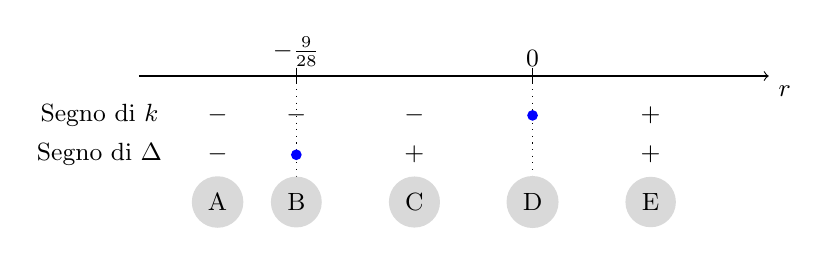
\begin{tikzpicture}[font=\small,x=10mm, y=10mm]

\draw[->] (0,0) -- (8,0) node [below right] () {$r$};

\foreach \x in {2,5}{
\draw(\x,3pt)--(\x,-3pt);
\begin{scope}[dotted]
\draw (\x,0) -- (\x,-1.5);
\end{scope}}
\node[] at (-.5,-0.5) {Segno di $k$};
\node[] at (-.5,-1) {Segno di $\Delta$};
\node[above]  at (2,0) {$-\frac{9}{28}$};
\node[above]  at (5,0) {$0$};
\node[] at (1,-0.5) {$-$};
\node[] at (2,-0.5) {$-$};
\node[] at (3.5,-0.5) {$-$};
\node[] at (6.5,-0.5) {$+$};
\node[] at (1,-1) {$-$};
\node[] at (3.5,-1) {$+$};
\node[] at (6.5,-1) {$+$};
\node [circle,fill=gray!30](A) at (1,-1.6) {A};
\node [circle,fill=gray!30](B) at (2,-1.6) {B};
\node [circle,fill=gray!30](C) at (3.5,-1.6) {C};
\node [circle,fill=gray!30](D) at (5,-1.6) {D};
\node [circle,fill=gray!30](E) at (6.5,-1.6) {E};

\begin{scope}[blue,thick]
\draw[fill=blue] (5,-.5)circle (1.5pt);
\draw[fill=blue] (2,-1)circle (1.5pt);
\end{scope}

\end{tikzpicture}

% % \end{center}
% \vspazio\ovalbox{\risolvii \ref{ese:4.1}, \ref{ese:4.2}, \ref{ese:4.3}, 
% \ref{ese:4.4}, \ref{ese:4.5}, \ref{ese:4.6}}
% 
% \end{esempio}
% 
% %%%%%%%%%%%%%%%%%%%%%%%%%%%%%%
% % \end{exrig}


\section{Disequazioni polinomiali di grado superiore}
\label{sec:diseq_grado_superiore}

\begin{procedura}
Risolvere le disequazioni di grado superiore:
\begin{enumeratea}
\item scomponi il polinomio di grado $n$ in fattori di primo e secondo grado;
\item studia il segno dei singoli fattori;
\item costruisci la tabella dei segni;
\item cerca gli intervalli in cui il polinomio dato assume il segno richiesto.
\item rappresenta, con i diversi metodi visti, gli intervalli che 
 risolvono la disequazione.
\end{enumeratea}
\end{procedura}

Applichiamo la procedura ai seguenti esempi.

% \begin{exrig}
\begin{esempio}
 \[p(x)=-2x^3+3x^2+8x-12 \le 0\]

In questo caso dobbiamo risolvere una disequazione di terzo grado. 
Possiamo ridurre la difficoltà scomponendo in fattori il polinomio in modo da 
ottenere il prodotto di più polinomi di primo grado: 

\begin{align*}
P(x) = -2x^3+3x^2+8x-12 &= x^2(-2x+3)-4(-2x+3) = \\
                        &= (x^2-4)(-2x+3)
\end{align*}

A questo punto possiamo studiare il segno dei fattori e, applicando la regola 
dei segni di un prodotto, trovare il segno del polinomio iniziale e risolvere 
la disequazione.

Studiamo il segno di ogni singolo fattore:
\begin{itemize}
 \item segno di \(x^2-4\)\\
 \begin{minipage}{.35\textwidth}
  E.A.:~\(x^2-4=0 \sRarrow x=\mp 2\)
 \end{minipage}
 \begin{minipage}{.25\textwidth}
  F.A.:~\(y=x^2-4 \sRarrow\)
 \end{minipage}
 \begin{minipage}{.38\textwidth}
  \begin{inaccessibleblock}[parabola concavità verso l'alto, interseca 
l'asse~x in -2 e +2]
  \parabolaamadma{-2}{+2}
\end{inaccessibleblock}
 \end{minipage}
 \item  segno di \(-2x+3\)\\
 \begin{minipage}{.35\textwidth}
  E.A.:~$-2x+3=0 \sRarrow x=\dfrac{3}{2}$
  \vspace{1.8em}
 \end{minipage}
 \begin{minipage}{.25\textwidth}
  F.A.:~$y=-2x+3 \sRarrow $
  \vspace{1.8em}
 \end{minipage}
 \begin{minipage}{.38\textwidth}
  \begin{inaccessibleblock}[retta decrescente con zero in~3/2]
%   \vspace*{1.7em}
  \rettammi{10}{\dfrac{3}{2}}
\end{inaccessibleblock}
 \end{minipage}
 \item Con la regola dei segni calcolo il segno del prodotto 
\begin{inaccessibleblock}[Grafo con i segni]
  \segnoprodotto
\end{inaccessibleblock}
%  \item Quindi i valori di~$x$ che rendono vera la disequazione, cioè i valori
%   che rendono~$f(x)$ non positivo, sono quelli 
%   che si trovano a sinistra di~$-2$ oppure che si trovano a destra di~$+3$. 
%  \subitem 
%   \begin{minipage}{.35\textwidth}
%    rappresentazione grafica: 
%   \end{minipage}
%   \begin{minipage}{.30\textwidth}
% \begin{inaccessibleblock}[Retta con gli intervalli evidenziati]
%    % (c) 2014 Daniele Zambelli - daniele.zambelli@gmail.com

%%%
% Valori esterni all'intervallo -2; 3
%%%%
 
\begin{tikzpicture}[x=1.5mm, y=1.5mm, smooth]

% \clip (-7.5, -5.5) rectangle (10.9, 10.9);

\coordinate (m_i) at (-10, 0);
\coordinate (a) at (-5, 0);
\coordinate (b) at (0, 0);
\coordinate (c) at (5, 0);
\coordinate (p_i) at (10, 0);

% (c) 2014 Daniele Zambelli - daniele.zambelli@gmail.com

%%%
% Asse cartesiano x
%%%%

% (c) 2014 Daniele Zambelli - daniele.zambelli@gmail.com

%%%
% Asse cartesiano generico
%%%%

\draw [-{Stealth[length=2mm, open, round]}] (-10, 0) -- (10, 0);

\node [below] at (10, 0)  {$x$};


\begin{scope}[blue,thick]
\draw [-,decorate,decoration=snake] (m_i) -- (a);
\draw[fill=white] (a) circle (2pt) node [above] {$-3$};
\draw [-,decorate,decoration=snake] (b) -- (c);
\draw[fill] (b) circle (2pt) node [above] {$\frac{1}{2}$};
\draw [fill=white] (c) -- (p_i);
\draw[fill] (c) circle (2pt) node [above] {$2$};
\end{scope}

\end{tikzpicture}

% \end{inaccessibleblock}
%   \end{minipage}
%  \subitem rappresentazione con i 
%    predicati:~$-2 \le x \le \frac{3}{2} \quad \lor \quad x \ge 2$ 
%  \subitem rappresentazione con le 
%   parentesi:~$]-2;~-3[ \quad \cup \quad [2;~+\infty]$. 
\end{itemize}

\end{esempio}

\begin{comment}

\begin{esempio}
Data la disequazione $-2x(3-2x)-3x^2\left(2-\frac 3 2x\right)\ge 
5\left(2x^2-\frac 3{10}x\right)$ determinate il suo $ \IS $

Osserviamo che la disequazione proposta è polinomiale di terzo grado; eseguiamo 
i calcoli per portarla alla forma $p(x)\ge 0$. Si ottiene $3x^3-8x^2-3x\ge 0$ e 
con la scomposizione \ si ha $x\cdot (3x^2-8x-3)\ge 0$. Procediamo con lo 
studio 
dei segni dei singoli fattori: $f_1\ge 0\rightarrow x\ge 0$ e $f_2\ge 
0\rightarrow x\le -\frac 1 3\vee x\ge 3$ e compiliamo \ la tabella dei segni 
che 
lasciamo al lettore.

\begin{center}
 % (c) 2013 Claudio Carboncini - claudio.carboncini@gmail.com
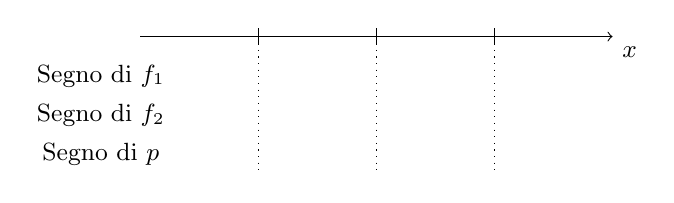
\begin{tikzpicture}[font=\small,x=10mm, y=10mm]

\draw[->] (0,0) -- (6,0) node [below right] () {$x$};

\foreach \x in {1.5,3,4.5}{
\draw(\x,3pt)--(\x,-3pt);
\begin{scope}[dotted]
\draw (\x,0) -- (\x,-1.7);
\end{scope}}
\node[] at (-.5,-0.5) {Segno di $f_1$};
\node[] at (-.5,-1) {Segno di $f_2$};
\node[] at (-.5,-1.5) {Segno di $p$};

\end{tikzpicture}

\end{center}
Otteniamo: $\IS=\left\{x\in \insR | -\frac 1 3\le x\le 0\vee x\ge 3\right\}$.
\end{esempio}

\begin{esempio}
Un numero è tale che sottraendo al suo cubo il suo triplo si ottiene un numero 
maggiore del triplo del suo quadrato aumentato di $ 4 $. Determinare l'insieme 
soluzione del problema.

La richiesta del problema implica la ricerca dell'Insieme Soluzione della 
disequazione $x^3-3x>3x^2+4$, di terzo grado nella variabile $x$. Scriviamo la 
disequazione in forma canonica, applicando i principi di equivalenza: 
$x^3-3x^2-3x-4>0$. Si tratta di una disequazione polinomiale di terzo grado.

Procediamo nella scomposizione in fattori del polinomio $p(x)=x^3-3x^2-3x-4$. 
Mediante la regola di Ruffini possiamo determinare un suo zero $x=4$ e dunque 
ottenere $p(x)=(x-4)(x^2+x+1)$.

Determiniamo il segno dei singoli fattori: primo fattore $f_1>0\to x>4$ secondo 
fattore $f_2>0\to x^2+x+1>0$ disequazione di secondo grado. Il primo 
coefficiente è positivo e il discriminante \ $\Delta =1-4=-3$ è negativo; la 
parabola volge la concavità verso l'alto e non ha zeri reali dunque il secondo 
fattore è positivo per qualunque valore reale di $x$. Costruiamo la tabella dei 
segni:

\begin{center}
 % (c) 2013 Claudio Carboncini - claudio.carboncini@gmail.com
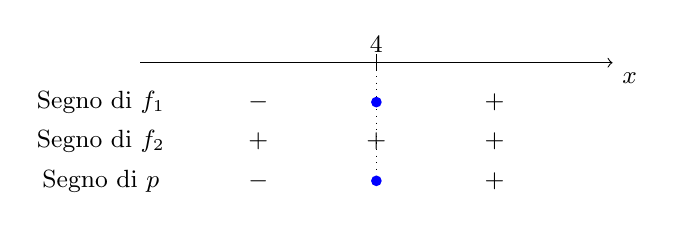
\begin{tikzpicture}[font=\small,x=10mm, y=10mm]

\draw[->] (0,0) -- (6,0) node [below right] () {$x$};

\draw(3,3pt)--(3,-3pt);
\begin{scope}[dotted]
\draw (3,0) -- (3,-1.5);
\end{scope}
\node[] at (-.5,-0.5) {Segno di $f_1$};
\node[] at (-.5,-1) {Segno di $f_2$};
\node[] at (-.5,-1.5) {Segno di $p$};
\node[above]  at (3,0) {$4$};
\node[] at (1.5,-0.5) {$-$};
\node[] at (4.5,-0.5) {$+$};
\node[] at (1.5,-1) {$+$};
\node[] at (3,-1) {$+$};
\node[] at (4.5,-1) {$+$};
\node[] at (1.5,-1.5) {$-$};
\node[] at (4.5,-1.5) {$+$};

\begin{scope}[blue,thick]
\draw[fill=blue] (3,-1.5)circle (1.5pt);
\draw[fill=blue] (3,-.5)circle (1.5pt);
\end{scope}

\end{tikzpicture}

\end{center}
$\IS=\{x\in \insR | x>4\}=(4;+\infty )$.
\end{esempio}

\begin{esempio}
Risolvere la disequazione: $64x^6-1<0$.

Il binomio al primo membro è una differenza di quadrati, quindi scomponendo si 
ottiene: $64x^6-1=(8x^3-1)(8x^3+1)=(2x-1)(4x^2+2x+1)(2x+1)(4x^2-2x+1)$.

Si tratta allora di studiare il segno dei singoli fattori: $f_1>0\to x>\frac 1 
2$ $f_2>0\to \forall x\in \insR$ $f_3>0\to x>-\frac 1 2$ $f_4>0\to \forall x\in 
\insR$ e di determinare il segno richiesto dopo aver costruito la tabella dei 
segni.
\end{esempio}

\begin{esempio}
Risolvere la disequazione: $x^4-4x^2-45>0$.

Il trinomio al primo membro è di quarto grado; sappiamo che con la sostituzione 
$x^2=t$ può essere ricondotto ad un trinomio di secondo grado la cui 
scomposizione in fattori risulta $(t-9)\cdot (t+5)$ e quindi la disequazione 
assegnata diventa: $(x^2-9)\cdot (x^2+5)>0$.

Si tratta allora di studiare il segno dei singoli fattori $f_1>0\to x<-3\vee 
x>3$ e $f_2>0\to \forall x\in \insR$ per poi determinare il segno richiesto 
dopo 
aver costruito la tabella dei segni.
\end{esempio}
% \end{exrig}
% \vspazio\ovalbox{\risolvii \ref{ese:4.32}, \ref{ese:4.33}, \ref{ese:4.34}, 
% \ref{ese:4.35}, \ref{ese:4.36}, \ref{ese:4.37}, \ref{ese:4.38}, 
% \ref{ese:4.39}, 
% \ref{ese:4.40}, \ref{ese:4.41}, \ref{ese:4.42}, \ref{ese:4.43}, \ref 
% {ese:4.44},}
% 
% \vspazio\ovalbox{\ref{ese:4.45}, \ref{ese:4.46}, \ref{ese:4.47}, 
% \ref{ese:4.48}, 
% \ref{ese:4.49}, \ref{ese:4.50}, \ref{ese:4.51}, \ref{ese:4.52}, 
% \ref{ese:4.53}, 
% \ref{ese:4.54}, \ref{ese:4.55}, \ref{ese:4.56}, \ref{ese:4.57}}

\newpage %----------------------------------------------

\section{Disequazioni fratte}
\label{sec:diseq_fratte}

Ricordiamo che una disequazione è \emph{frazionaria} o \emph{fratta} quando il 
suo denominatore contiene l'incognita. Per risolverla si può applicare la 
seguente

\begin{procedura}
Soluzione di una disequazione frazionaria:
\begin{enumeratea}
\item trasporta tutti i termini al primo membro e scrivilo sotto forma di 
 un'unica frazione: $\frac{N(x)}{D(x)} \lessgtr 0$;
% \item si determinano le Condizioni di Esistenza ponendo $D(x)\neq 0$
% \item impostiamo la disequazione nella forma $\frac{N(x)}{D(x)}\ge 0$ oppure 
% $\frac{N(x)}{D(x)}\le 0$ oppure $\frac{N(x)}{D(x)}<0$ oppure 
% $\frac{N(x)}{D(x)}>0$ a seconda del quesito posto da problema;
\item scomponi in fattori numeratore e denominatore;
\item studia il segno di ogni fattore;
\item costruisci la tabella dei segni, ricordandosi di indicare con una 
 crocetta gli zeri del denominatore;
\item applica la regola dei segni per calcolare il segno della frazione;
\item individuano gli intervalli in cui la frazione assume il segno richiesto;
\item rappresenta, con i diversi metodi visti, gli intervalli che 
 risolvono la disequazione.
\end{enumeratea}
\end{procedura}

Vediamo attraverso alcuni esempi come procedere.

 \begin{esempio}
\[\frac{2}{x-7} \ge \frac{3}{x+4}\]
\begin{itemize}
 \item Scrivere la disequazione in forma normale:
 \[\frac{2}{x-7} - \frac{3}{x+4} \ge 0 \Rightarrow 
   \frac{2 x +8 -3x +21}{(x-7)(x+4)} \ge 0 \Rightarrow
   \frac{-x +29}{(x-7)(x+4)} \ge 0\]
 \item Segno del numeratore:\\
 \begin{minipage}{.45\textwidth}
  E.A.:~$-x +29=0 \Rightarrow x=29$
 \end{minipage}
 \begin{minipage}{.25\textwidth}
  F.A.:~$y=-x +29 \rightarrow $
 \end{minipage}
 \begin{minipage}{.3\textwidth}
  % (c) 2014 Daniele Zambelli - daniele.zambelli@gmail.com

%%%
% Retta decrescente zero in 3
%%%%
 
\begin{tikzpicture}[x=1.5mm, y=1.5mm, smooth]

% (c) 2014 Daniele Zambelli - daniele.zambelli@gmail.com

%%%
% Retta decrescente con segni
%%%%
 
\coordinate (inizio) at (-10, 4);
\coordinate (zero) at (0, 0);
\coordinate (fine) at (10, -4);

% (c) 2014 Daniele Zambelli - daniele.zambelli@gmail.com

%%%
% Asse cartesiano x
%%%%

\input{lbr/assiepiani/asse10.pgf}
\node [below] at (10, 0)  {$x$};


\draw [-] [ultra thick, blue!50!black] (inizio) -- (zero);
\draw [-] [ultra thick, red!50!black] (zero) -- (fine);

\node [xshift=-25, yshift=-3, above] at (zero) {$+$};
\draw[blue, thick, fill=white] (zero) circle (2pt);
\node [xshift=25, yshift=-3, above] at (zero) {$-$};

\node [above] {$+29$};

\end{tikzpicture}

 \end{minipage}
 \item Segno del denominatore 1:\\
 \begin{minipage}{.45\textwidth}
  E.A.:~$x -7=0 \Rightarrow x=+7$
 \end{minipage}
 \begin{minipage}{.25\textwidth}
  F.A.:~$y=x -7 \rightarrow $
 \end{minipage}
 \begin{minipage}{.3\textwidth}
  % (c) 2014 Daniele Zambelli - daniele.zambelli@gmail.com

%%%
% Retta crescente zero in -2
%%%%
 
\begin{tikzpicture}[x=1.5mm, y=1.5mm, smooth]

% (c) 2014 Daniele Zambelli - daniele.zambelli@gmail.com

%%%
% Retta crescente con segni
%%%%
 
\coordinate (inizio) at (-10, -4);
\coordinate (zero) at (0, 0);
\coordinate (fine) at (10, 4);

% (c) 2014 Daniele Zambelli - daniele.zambelli@gmail.com

%%%
% Asse cartesiano x
%%%%

\input{lbr/assiepiani/asse10.pgf}
\node [below] at (10, 0)  {$x$};


\draw [-] [ultra thick, red!50!black] (inizio) -- (zero);
\draw [-] [ultra thick, blue!50!black] (zero) -- (fine);

\node [xshift=-25, yshift=-3, above] at (zero) {$-$};
\draw[blue, thick, fill=white] (zero) circle (2pt);
\node [xshift=25, yshift=-3, above] at (zero) {$+$};

\node [above] {$+7$};

\end{tikzpicture}

 \end{minipage}
 \item Segno del denominatore 2:\\
 \begin{minipage}{.45\textwidth}
  E.A.:~$x +4=0 \Rightarrow x=-4$
 \end{minipage}
 \begin{minipage}{.25\textwidth}
  F.A.:~$y=x +4 \rightarrow $
 \end{minipage}
 \begin{minipage}{.3\textwidth}
  % (c) 2014 Daniele Zambelli - daniele.zambelli@gmail.com

%%%
% Retta crescente zero in -2
%%%%
 
\begin{tikzpicture}[x=1.5mm, y=1.5mm, smooth]

% (c) 2014 Daniele Zambelli - daniele.zambelli@gmail.com

%%%
% Retta crescente con segni
%%%%
 
\coordinate (inizio) at (-10, -4);
\coordinate (zero) at (0, 0);
\coordinate (fine) at (10, 4);

% (c) 2014 Daniele Zambelli - daniele.zambelli@gmail.com

%%%
% Asse cartesiano x
%%%%

\input{lbr/assiepiani/asse10.pgf}
\node [below] at (10, 0)  {$x$};


\draw [-] [ultra thick, red!50!black] (inizio) -- (zero);
\draw [-] [ultra thick, blue!50!black] (zero) -- (fine);

\node [xshift=-25, yshift=-3, above] at (zero) {$-$};
\draw[blue, thick, fill=white] (zero) circle (2pt);
\node [xshift=25, yshift=-3, above] at (zero) {$+$};

\node [above] {$-4$};

\end{tikzpicture}

 \end{minipage}
 \item Con la regola dei segni calcolo il segno della frazione 
  % (c) 2014 Daniele Zambelli - daniele.zambelli@gmail.com

%%%
% Studio dei segni di una frazione
%%%%
 
\begin{tikzpicture}[x=2.5mm, y=5mm, smooth]

\coordinate (a_top) at (-5, 1);
\coordinate (a_bottom) at (-5, -3);
\coordinate (b_top) at (0, 1);
\coordinate (b_bottom) at (0, -3);
\coordinate (c_top) at (5, 1);
\coordinate (c_bottom) at (5, -3);

% (c) 2014 Daniele Zambelli - daniele.zambelli@gmail.com

%%%
% Grafo per il calcolo del segno con tre assi
%%%%
 
% (c) 2014 Daniele Zambelli - daniele.zambelli@gmail.com

%%%
% Asse cartesiano x
%%%%

\input{lbr/assiepiani/asse10.pgf}
\node [below] at (10, 0)  {$x$};

\begin{scope}[yshift= -.5cm]
  % (c) 2014 Daniele Zambelli - daniele.zambelli@gmail.com

%%%
% Asse cartesiano x
%%%%

\input{lbr/assiepiani/asse10.pgf}
\node [below] at (10, 0)  {$x$};

  \begin{scope}[yshift= -.5cm]
    % (c) 2014 Daniele Zambelli - daniele.zambelli@gmail.com

%%%
% Asse cartesiano x
%%%%

\input{lbr/assiepiani/asse10.pgf}
\node [below] at (10, 0)  {$x$};

    \begin{scope}[yshift= -.5cm]
      % (c) 2014 Daniele Zambelli - daniele.zambelli@gmail.com

%%%
% Asse cartesiano x
%%%%

\input{lbr/assiepiani/asse10.pgf}
\node [below] at (10, 0)  {$x$};

    \end{scope}
  \end{scope}
\end{scope}

\draw [-] [] (a_top) -- (a_bottom);
\draw [-] [] (b_top) -- (b_bottom);
\draw [-] [] (c_top) -- (c_bottom);

\node [above] at (-5, 1) {$-4$};
\node [above] at (0, 1) {$+7$};
\node [above] at (5, 1) {$+29$};

\node [above left] at (-10, 0) {$-x+29$};
\node [above] at (-7.5, 0) {$+$};
\node [above] at (-2.5, 0) {$+$};
\node [above] at (2.5, 0) {$+$};
\draw (5, .5) circle (3pt);
\node [above] at (7.5, 0) {$-$};

\node [above left] at (-10, -1) {$x-7$};
\node [above] at (-7.5, -1) {$-$};
\node [above] at (-2.5, -1) {$-$};
\draw (0 -.4, -0.5 -.2) -- (0 +.4, -0.5 +.2) 
      (0 -.4, -0.5 +.2) -- (0 +.4, -0.5 -.2);
\node [above] at (2.5, -1) {$+$};
\node [above] at (7.5, -1) {$+$};

\node [above left] at (-10, -2) {$x+4$};
\node [above] at (-7.5, -2) {$-$};
\draw (-5 -.4, -1.5 -.2) -- (-5 +.4, -1.5 +.2) 
      (-5 -.4, -1.5 +.2) -- (-5 +.4, -1.5 -.2);
\node [above] at (-2.5, -2) {$+$};
\node [above] at (2.5, -2) {$+$};
\node [above] at (7.5, -2) {$+$};

\node [above left] at (-10, -3.15) {$F(x)$};
\node [above] at (-7.5, -3) {$+$};
\draw (-5 -.4, -2.5 -.2) -- (-5 +.4, -2.5 +.2) 
      (-5 -.4, -2.5 +.2) -- (-5 +.4, -2.5 -.2);
\node [above] at (-2.5, -3) {$-$};
\draw (0 -.4, -2.5 -.2) -- (0 +.4, -2.5 +.2) 
      (0 -.4, -2.5 +.2) -- (0 +.4, -2.5 -.2);
\node [above] at (2.5, -3) {$+$};
\draw (5, -2.5) circle (3pt);
\node [above] at (7.5, -3) {$-$};

\end{tikzpicture}
 
 \item Quindi i valori di~$x$ che rendono vera la disequazione, cioè i valori
  che rendono~$f(x)$ negativo, sono quelli 
  che si trovano a sinistra di~$-2$ oppure che si trovano a destra di~$+3$. 
 \subitem 
  \begin{minipage}{.35\textwidth}
   rappresentazione grafica: 
  \end{minipage}
  \begin{minipage}{.30\textwidth}
   % (c) 2014 Daniele Zambelli - daniele.zambelli@gmail.com

%%%
% Valori x < -4  or  7 < x <= 29
%%%%
 
\begin{tikzpicture}[x=1.5mm, y=1.5mm, smooth]

% \clip (-7.5, -5.5) rectangle (10.9, 10.9);

\coordinate (m_i) at (-10, 0);
\coordinate (a) at (-5, 0);
\coordinate (b) at (0, 0);
\coordinate (c) at (5, 0);
\coordinate (p_i) at (10, 0);

% (c) 2014 Daniele Zambelli - daniele.zambelli@gmail.com

%%%
% Asse cartesiano x
%%%%

% (c) 2014 Daniele Zambelli - daniele.zambelli@gmail.com

%%%
% Asse cartesiano generico
%%%%

\draw [-{Stealth[length=2mm, open, round]}] (-10, 0) -- (10, 0);

\node [below] at (10, 0)  {$x$};


\begin{scope}[blue,thick]
\draw [-,decorate,decoration=snake] (m_i) -- (a);
% \draw[fill=white] (a) circle (2pt) node [above] {$-3$};
\draw[fill=white] (a) circle (2pt) node [above] {$-4$};
% \draw [-,decorate,decoration=snake] (b) -- (c);
\draw[fill=white] (b) circle (2pt) node [above] {$+7$};
\draw [decorate,decoration=snake] (b) -- (c);
\draw[fill] (c) circle (2pt) node [above] {$+29$};
\end{scope}

\end{tikzpicture}

  \end{minipage}
 \subitem rappresentazione con i 
  predicati:~$x < -4 \quad \lor \quad +7 < x \le 29$ 
 \subitem rappresentazione con le 
  parentesi:~$]-\infty;~-4[ \quad \cup \quad ]+7;~+\infty[$. 
\end{itemize}
 \end{esempio}

% \begin{exrig}
\begin{esempio}
Data l'espressione $E=\frac 4{4x^2-1}+\frac 1{2x+1}+\frac x{1-2x}$ 
determinarne, 
al variare di $x$ in $\insR$, il segno.

\emph{Osservazioni preliminari}
\begin{itemize*}
\item L'espressione assegnata è frazionaria, quindi lo studio del segno deve 
essere circoscritto ai valori di $x$ del Dominio dell'espressione stessa;
\item studiare il segno di una espressione letterale significa stabilire in 
quale insieme si trovano i valori della variabile che la rendono positiva, 
negativa, nulla;
\item ogni espressione contenente operazioni tra frazioni algebriche ha in 
generale come risultato una frazione algebrica.
\end{itemize*}

\emph{Strategia risolutiva}
\begin{enumeratea}
\item determiniamo il risultato dell'operazione assegnata: 
$E=\frac{-2x^2+x+3}{(2x+1)\cdot (2x-1)}$
\item determiniamo il dominio: $\CE\, 2x+1\neq 0\wedge 2x-1\neq 0\to 
D=\insR-\left\{-\frac 1 2,\frac 1 2\right\}$
\item impostiamo la disequazione: $\frac{-2x^2+x+3}{(2x+1)\cdot (2x-1)}\ge 0$ 
che ci permetterà di rispondere al quesito posto dal problema;
\item studiamo il segno di numeratore e denominatore:
 \begin{itemize*}
\item segno $N: -2x^2+x+3\ge 0$ disequazione di secondo grado, quindi 
dall'equazione associata $-2x^2+x+3=0$, calcoliamo il discriminante: $\Delta 
=1+24=25$, positivo per cui si hanno due soluzioni reali distinte; la parabola 
$y=-2x^2+x+3$ ha concavità verso il basso per cui essendo $x_1=-1$ e $x_2=\frac 
3 2$ si ha $N\ge 0$ per $-1\le x\le \frac 3 2$
\item segno $D$: il denominatore è composto da due fattori di primo grado, 
quindi $d_1>0$ per $x>-\frac 1 2$ e $d_2>0$ per $x>\frac 1 2$
 \end{itemize*}
\item costruiamo la tabella dei segni:

\begin{center}
 % (c) 2013 Claudio Carboncini - claudio.carboncini@gmail.com
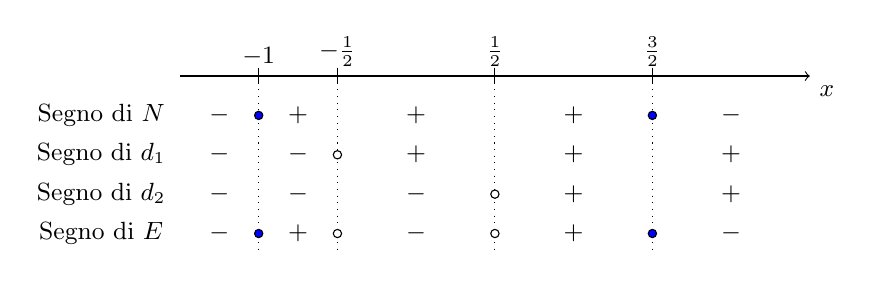
\begin{tikzpicture}[font=\small,x=10mm, y=10mm]

\draw[->] (0,0) -- (8,0) node [below right] () {$x$};

\foreach \x in {1,2,4,6}{
\draw(\x,3pt)--(\x,-3pt);
\begin{scope}[dotted]
\draw (\x,0) -- (\x,-2.2);
\end{scope}}
\node[] at (-1,-0.5) {Segno di $N$};
\draw[fill=blue] (1,-.5)circle (1.5pt);
\draw[fill=blue] (6,-.5)circle (1.5pt);
\node[] at (-1,-1) {Segno di $d_1$};
\draw[fill=white] (2,-1)circle (1.5pt);
\node[] at (-1,-1.5) {Segno di $d_2$};
\draw[fill=white] (4,-1.5)circle (1.5pt);
\node[] at (-1,-2) {Segno di $E$};
\draw[fill=blue] (1,-2)circle (1.5pt);
\draw[fill=blue] (6,-2)circle (1.5pt);
\draw[fill=white] (2,-2)circle (1.5pt);
\draw[fill=white] (4,-2)circle (1.5pt);
\node[above]  at (1,0) {$-1$};
\node[above]  at (2,0) {$-{\frac{1}{2}}$};
\node[above]  at (4,0) {${\frac{1}{2}}$};
\node[above]  at (6,0) {${\frac{3}{2}}$};
\node[] at (.5,-0.5) {$-$};
\node[] at (1.5,-0.5) {$+$};
\node[] at (3,-0.5) {$+$};
\node[] at (5,-0.5) {$+$};
\node[] at (7,-0.5) {$-$};
\node[] at (.5,-1) {$-$};
\node[] at (1.5,-1) {$-$};
\node[] at (3,-1) {$+$};
\node[] at (5,-1) {$+$};
\node[] at (7,-1) {$+$};
\node[] at (.5,-1.5) {$-$};
\node[] at (1.5,-1.5) {$-$};
\node[] at (3,-1.5) {$-$};
\node[] at (5,-1.5) {$+$};
\node[] at (7,-1.5) {$+$};
\node[] at (.5,-2) {$-$};
\node[] at (1.5,-2) {$+$};
\node[] at (3,-2) {$-$};
\node[] at (5,-2) {$+$};
\node[] at (7,-2) {$-$};

\end{tikzpicture}

\end{center}
\item dalla tabella dei segni possiamo ottenere la risposta al problema posto:
\begin{itemize*}
\item l'espressione $E$ si annulla per $x=-1\vee x=\frac 3 2$
\item l'espressione $E$ è positiva per $x\in A=\left\{x\in \insR | -1<x<-\frac 
1 
2\vee \frac 1 2<x<\frac 3 2\right\}$
\item l'espressione $E$ è negativa per $x\in B=\left\{x\in \insR | x<-1\vee 
-\frac 1 2<x<\frac 1 2\vee x>\frac 3 2\right\}$.
\end{itemize*}
\end{enumeratea}
\end{esempio}

\begin{esempio}
Determiniamo l'Insieme Soluzione della disequazione fratta: $3-\frac 1{2x+1}\ge 
\frac 1{1-x}$.
\begin{enumeratea}
\item Trasportiamo al primo membro la frazione del secondo membro $E=3-\frac 
1{2x+1}-\frac 1{1-x}$ ed eseguiamo i calcoli ottenendo: 
$E=\frac{-6x^2+2x+1}{(2x+1)\cdot (1-x)}$
\item determiniamo il dominio: $\CE \;2x+1\neq 0\wedge 1-x\neq 0\to 
D=\insR-\left\{-\frac 1 2,1\right\}$
\item impostiamo la disequazione: \ $\frac{-6x^2+2x+1}{(2x+1)\cdot (1-x)}\ge 0$ 
che ci permetterà di rispondere al quesito posto dal problema;
\item studiamo il segno del numeratore e del denominatore:
\begin{itemize*}
\item segno N: $-6x^2+2x+1\ge 0$ disequazione di secondo grado, quindi scritta 
l'equazione associata $-6x^2+2x+1=0$, calcoliamone il discriminante: 
$\frac{\Delta } 4=7$, positivo per cui si hanno due soluzioni 
$x_{1,2}=\frac{1\pm \sqrt 7} 6$ essendo il primo coefficiente negativo si ha 
$N\ge 0$ per $\frac{1-\sqrt 7} 6\le x\le \frac{1+\sqrt 7} 6$
\item segno D: $-2x^2+x+1>0$ disequazione di secondo grado; il denominatore ha 
due zeri reali $x=-\frac 1 2$ e $x_2=1$, il primo coefficiente è negativo, 
pertanto $D>0$ per $-\frac 1 2<x<1$ che rispetta le C.E.: $x_1\neq -\frac 1 
2\wedge x_2\neq 1$
\end{itemize*}
\item compiliamo la tabella dei segni:

\begin{center}
 % (c) 2013 Claudio Carboncini - claudio.carboncini@gmail.com
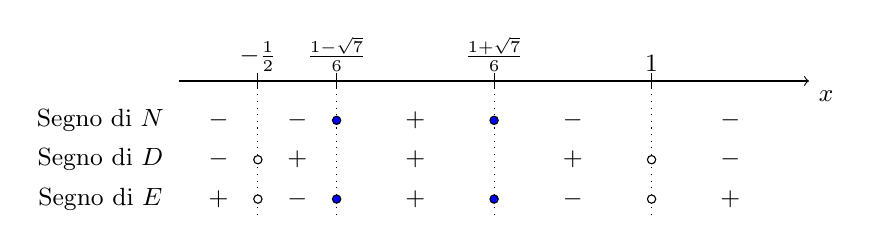
\begin{tikzpicture}[font=\small,x=10mm, y=10mm]

\draw[->] (0,0) -- (8,0) node [below right] () {$x$};

\foreach \x in {1,2,4,6}{
\draw(\x,3pt)--(\x,-3pt);
\begin{scope}[dotted]
\draw (\x,0) -- (\x,-1.7);
\end{scope}}

\node[] at (-1,-0.5) {Segno di $N$};
\draw[fill=blue] (2,-.5)circle (1.5pt);
\draw[fill=blue] (4,-.5)circle (1.5pt);
\node[] at (-1,-1) {Segno di $D$};
\draw[fill=white] (1,-1)circle (1.5pt);
\draw[fill=white] (6,-1)circle (1.5pt);
\node[] at (-1,-1.5) {Segno di $E$};
\draw[fill=blue] (2,-1.5)circle (1.5pt);
\draw[fill=blue] (4,-1.5)circle (1.5pt);
\draw[fill=white] (1,-1.5)circle (1.5pt);
\draw[fill=white] (6,-1.5)circle (1.5pt);
\node[above]  at (1,0) {$-{\frac{1}{2}}$};
\node[above]  at (2,0) {${\frac{1-\sqrt{7}}{6}}$};
\node[above]  at (4,0) {${\frac{1+\sqrt{7}}{6}}$};
\node[above]  at (6,0) {$1$};
\node[] at (.5,-0.5) {$-$};
\node[] at (1.5,-0.5) {$-$};
\node[] at (3,-0.5) {$+$};
\node[] at (5,-0.5) {$-$};
\node[] at (7,-0.5) {$-$};
\node[] at (.5,-1) {$-$};
\node[] at (1.5,-1) {$+$};
\node[] at (3,-1) {$+$};
\node[] at (5,-1) {$+$};
\node[] at (7,-1) {$-$};
\node[] at (.5,-1.5) {$+$};
\node[] at (1.5,-1.5) {$-$};
\node[] at (3,-1.5) {$+$};
\node[] at (5,-1.5) {$-$};
\node[] at (7,-1.5) {$+$};

\end{tikzpicture}

\end{center}
\item determiniamo l'insieme soluzione: $\IS=\left\{x\in \insR | x<-\frac 1 
2\vee \frac{1-\sqrt 7} 6\le x\le \frac{1+\sqrt 7} 6\vee x>1\right\}$.
\end{enumeratea}
\end{esempio}
% \end{exrig}

% \vspazio\ovalbox{\risolvii \ref{ese:4.58}, \ref{ese:4.59}, \ref{ese:4.60}, 
% \ref{ese:4.61}, \ref{ese:4.62}, \ref{ese:4.63}, \ref{ese:4.64}, 
% \ref{ese:4.65}, 
% \ref{ese:4.66}, \ref{ese:4.67}, \ref{ese:4.68}, \ref{ese:4.69}, \ref 
% {ese:4.70},}
% 
% \vspazio\ovalbox{\ref{ese:4.71}, \ref{ese:4.72}, \ref{ese:4.47}, 
% \ref{ese:4.73}, 
% \ref{ese:4.74}}

\section{Sistemi di disequazioni}
\label{sec:diseq_sistemi}

Ricordiamo che risolvere un sistema di disequazioni significa trovare l'insieme 
dei numeri reali che sono le soluzioni comuni alle disequazioni che lo 
compongono. Indicate con $d_{1}, d_{2}, \ldots, d_n$ le disequazioni che 
formano 
il sistema e $\IS_{1}, \IS_{2}, \ldots,\IS_n$ i rispettivi insieme soluzione, 
la 
soluzione del sistema indicata con $\IS$ è data da $\IS=\IS_1\cap 
\IS_{2,}\ldots 
\cap \IS_n$.

\begin{problema}
Nell'equazione $x^2-(k-3)x+k^2-3k+1=0$, determinare per quali valori del 
parametro $ k $ si ottengono soluzioni reali e concordi.
\end{problema}
Abbiamo già affrontato un \ problema di questo tipo discutendo le equazioni 
parametriche di secondo grado e dunque sappiamo che la richiesta del problema 
esige che il discriminante $(\Delta )$ sia non negativo affinché le soluzioni 
siano reali e che il prodotto delle stesse sia positivo. Pertanto il problema è 
formalizzato con un sistema di disequazioni: $\left\{\begin{array}{l}{\Delta 
\ge 
0}\\{\frac c a>0}\end{array}\right. \to 
\left\{\begin{array}{l}{k^2-6k+9-4k^2+12k-4\ge 
0}\\{k^2-3k+1>0}\end{array}\right.$.

Risolviamo separatamente le due disequazioni del sistema; indicati con $\IS_1$ 
e 
$\IS_2$ rispettivamente gli insiemi soluzione della prima e della seconda 
disequazione, l'insieme soluzione del sistema è dato da $\IS=\IS_1\cap \IS_2$ 
(insieme intersezione degli insiemi soluzione delle due disequazioni).
\begin{itemize*}
\item $d_1$: $-3k^2+6k+5\ge 0$ disequazione di secondo grado avente primo 
coefficiente negativo e $\frac{\Delta } 4=24$ positivo; la parabola 
$y=-3k^2+6k+5\ge 0$ ha concavità verso il basso e discriminante positivo, per 
cui essendo $x_1=\frac{3-2\sqrt 6} 3\vee x_2=\frac{3+2\sqrt 6} 3$ si ottiene 
$\IS_1=\left\{x\in \insR | \frac{3-2\sqrt 6} 3\le x\le \frac{3+2\sqrt 6} 
3\right\}$.
\item $d_2$: $k^2-3k+1>0$ disequazione di secondo grado avente il primo 
coefficiente positivo e $\Delta =5$ positivo; la parabola $y=k^2-3k+1>0$ ha 
concavità verso l'alto e discriminante positivo, quindi $x_1=\frac{3-\sqrt 5} 
2\vee x_2=\frac{3+\sqrt 5} 2$ e
$\IS_2=~\left\{x\in \insR | x<\frac{3-\sqrt 5} 2\vee x>\frac{3+\sqrt 5} 
2\right\}$.
\end{itemize*}
Per determinare l'Insieme Soluzione del sistema rappresentiamo in un grafico 
gli 
insiemi soluzioni delle disequazioni risolte e visualizziamo l'insieme formato 
dai valori che soddisfano contemporaneamente sia l'una che l'altra: sull'asse 
reale depositiamo i valori numerici trovati e rappresentiamo su righe distinte 
i 
due insiemi soluzione: gli intervalli in cui cadono soluzioni della prima e 
della seconda disequazione rappresentano l'Insieme Soluzione del sistema.

\begin{center}
 % (c) 2013 Claudio Carboncini - claudio.carboncini@gmail.com
\begin{tikzpicture}[font=\small,x=10mm, y=10mm]

\draw[->] (0,0) -- (8,0) node [below right] () {$r$};

\foreach \x in {2,3.5,5,6.5}{
\draw(\x,3pt)--(\x,-3pt);
\begin{scope}[dotted]
\draw (\x,0) -- (\x,-2);
\draw (0,-.5) -- (2,-.5);
\draw (6.5,-.5) -- (8,-.5);
\draw (3.5,-1) -- (5,-1);
\draw (0,-1.5) -- (2,-1.5);
\draw (3.5,-1.5) -- (5,-1.5);
\draw (6.5,-1.5) -- (8,-1.5);
\end{scope}}

\node[above]  at (2,0) {$\frac{3-2 \sqrt{6}}{3}$};
\node[above]  at (3.5,0) {$\frac{3- \sqrt{5}}{2}$};
\node[above]  at (5,0) {$\frac{3+ \sqrt{5}}{2}$};
\node[above]  at (6.5,0) {$\frac{3+2 \sqrt{6}}{3}$};
\pattern[pattern= north east lines, pattern color=red] (2,-2) rectangle (3.5,-1.5);
\pattern[pattern= north east lines, pattern color=red] (5,-2) rectangle (6.5,-1.5);

\node[] () at (-.5,-.5) {$\IS_{1}$};
\node[] () at (-.5,-1) {$\IS_{2}$};
\node[] () at (-.5,-1.75) {$\IS$};

\begin{scope}[blue,thick]
\draw (2,-.5) -- (6.5,-.5);
\draw (0,-1) -- (3.5,-1);
\draw (5,-1) -- (8,-1);
\draw (2,-1.5) -- (3.5,-1.5);
\draw (5,-1.5) -- (6.5,-1.5);

\draw[fill=blue] (2,-.5)circle (1.5pt);
\draw[fill=blue] (6.5,-.5)circle (1.5pt);
\draw[fill=white] (3.5,-1)circle (1.5pt);
\draw[fill=white] (5,-1)circle (1.5pt);
\draw[fill=blue] (2,-1.5)circle (1.5pt);
\draw[fill=blue] (6.5,-1.5)circle (1.5pt);
\draw[fill=white] (3.5,-1.5)circle (1.5pt);
\draw[fill=white] (5,-1.5)circle (1.5pt);

\end{scope}

\end{tikzpicture}

\end{center}

$\IS_1=\left\{x\in \insR\left|\frac{3-2\sqrt 6} 3\le x<\frac{3-\sqrt 5} 2\vee 
\frac{3+\sqrt 5} 2<x\le \frac{3+2\sqrt 6} 3\right.\right\}$

o scritto utilizzando gli intervalli: 

$\left.\left[\frac{3-2\sqrt 6} 3;\frac{3-\sqrt 5} 
2\right.\right[ \cup \left.\left]\frac{3+\sqrt 5} 2;\frac{3+2\sqrt 6} 
3\right.\right]$.

\begin{problema}
Risolvere il seguente sistema di disequazioni: $ 
\left\{\begin{array}{l}2x^3-9x^2+10x-3\le 0\\ \frac{x^2+x+1}{\ x^3-x}\ge 0 
\\3-4x<0 \end{array}\right.$.
\end{problema}
Il sistema è formato da tre disequazioni; risolviamo separatamente ciascuna 
disequazione:

\begin{itemize*}
\item $d_1$: $2x^3-9x^2+10x-3\le 0$ di terzo grado, scomponiamo in fattori. 
$x=1$ è uno zero del polinomio quindi con la regola di Ruffini otteniamo $d_1$: 
$(x-1)\cdot (2x^2-7x+3)\le 0$. L'equazione di secondo grado $2x^2-7x+3=0$ ha 
soluzioni reali $x_1=\frac 1 2\vee x=3$. Si tratta allora di studiare il segno 
dei singoli fattori e di determinare il segno richiesto dopo aver costruito la 
tabella dei segni:

\begin{center}
 % (c) 2013 Claudio Carboncini - claudio.carboncini@gmail.com
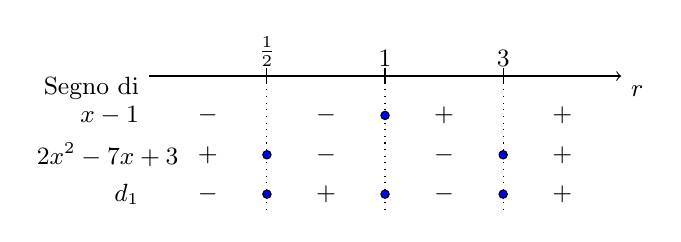
\begin{tikzpicture}[font=\small,x=10mm, y=10mm]

\draw[->] (0,0) -- (6,0) node [below right] () {$r$};

\foreach \x in {1.5,3,4.5}{
\draw(\x,3pt)--(\x,-3pt);
\begin{scope}[dotted]
\draw (\x,0) -- (\x,-1.7);
\end{scope}}

\node[left] at (0,-0.15) {Segno di};
\node[left] at (0,-0.5) {$x-1$};
\node[left] at (.5,-1) {$2x^2-7x+3$};
\node[left] at (0,-1.5) {$d_1$};
\node[above]  at (1.5,0) {$\frac{1}{2}$};
\node[above]  at (3,0) {$1$};
\node[above]  at (4.5,0) {$3$};
\node[] at (.75,-0.5) {$-$};
\node[] at (2.25,-0.5) {$-$};
\node[] at (3.75,-0.5) {$+$};
\node[] at (5.25,-0.5) {$+$};
\node[] at (.75,-1) {$+$};
\node[] at (2.25,-1) {$-$};
\node[] at (3.75,-1) {$-$};
\node[] at (5.25,-1) {$+$};
\node[] at (.75,-1.5) {$-$};
\node[] at (2.25,-1.5) {$+$};
\node[] at (3.75,-1.5) {$-$};
\node[] at (5.25,-1.5) {$+$};

\draw[fill=blue] (3,-.5)circle (1.5pt);
\draw[fill=blue] (1.5,-1)circle (1.5pt);
\draw[fill=blue] (4.5,-1)circle (1.5pt);
\draw[fill=blue] (3,-1.5)circle (1.5pt);
\draw[fill=blue] (1.5,-1.5)circle (1.5pt);
\draw[fill=blue] (4.5,-1.5)circle (1.5pt);

\end{tikzpicture}

\end{center}
L'insieme soluzione, tenendo conto che cerchiamo i valori per i quali $d_1$ 
risulta minore o uguale a $0$ è $\IS_1=\left\{x\in \insR | x\le\frac 1 2\vee 
1\le x\le 3\right\}$.

\item $d_2$: $\frac{x^2+x+1}{x^3-x}\ge 0$ è una disequazione fratta, per prima 
cosa scomponiamo in fattori il denominatore: $\frac{x^2+x+1}{x(x^2-1)}\ge 0$.
Studiamo poi il segno dei singoli fattori o divisori, tenendo conto che 
$x^2+x+1=0$ ha $\Delta <0$, per cui $x^2+x+1$ è sempre positivo.

\begin{center}
 % (c) 2013 Claudio Carboncini - claudio.carboncini@gmail.com
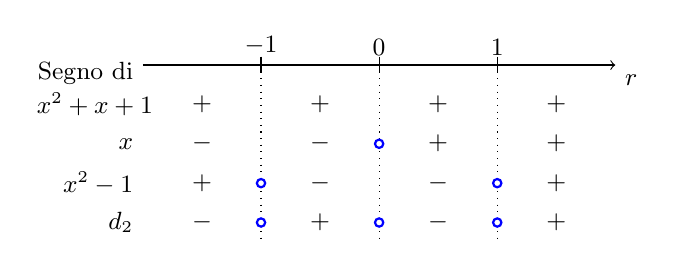
\begin{tikzpicture}[font=\small,x=10mm, y=10mm]

\draw[->] (0,0) -- (6,0) node [below right] () {$r$};

\foreach \x in {1.5,3,4.5}{
\draw(\x,3pt)--(\x,-3pt);
\begin{scope}[dotted]
\draw (\x,0) -- (\x,-2.2);
\end{scope}}

\node[left] at (0,-0.1) {Segno di};
\node[left] at (.25,-0.5) {$x^2+x+1$};
\node[left] at (0,-1) {$x$};
\node[left] at (0,-1.5) {$x^2-1$};
\node[left] at (0,-2) {$d_2$};
\node[above]  at (1.5,0) {$-1$};
\node[above]  at (3,0) {$0$};
\node[above]  at (4.5,0) {$1$};
\node[] at (.75,-0.5) {$+$};
\node[] at (2.25,-0.5) {$+$};
\node[] at (3.75,-0.5) {$+$};
\node[] at (5.25,-0.5) {$+$};
\node[] at (.75,-1) {$-$};
\node[] at (2.25,-1) {$-$};
\node[] at (3.75,-1) {$+$};
\node[] at (5.25,-1) {$+$};
\node[] at (.75,-1.5) {$+$};
\node[] at (2.25,-1.5) {$-$};
\node[] at (3.75,-1.5) {$-$};
\node[] at (5.25,-1.5) {$+$};
\node[] at (.75,-2) {$-$};
\node[] at (2.25,-2) {$+$};
\node[] at (3.75,-2) {$-$};
\node[] at (5.25,-2) {$+$};

\begin{scope}[blue,thick]
\draw[fill=white] (3,-1)circle (1.5pt);
\draw[fill=white] (1.5,-1.5)circle (1.5pt);
\draw[fill=white] (4.5,-1.5)circle (1.5pt);
\draw[fill=white] (3,-2)circle (1.5pt);
\draw[fill=white] (1.5,-2)circle (1.5pt);
\draw[fill=white] (4.5,-2)circle (1.5pt);
\end{scope}

\end{tikzpicture}

\end{center}
L'insieme soluzione, per $d_2\ge 0$ è $\IS_2=\left\{x\in \insR | -1<x<0\vee 
x>1\right\}$.
\item $d_3:3-4x<0$ è di primo grado per cui l'insieme soluzione è 
$\IS_3=\left\{x\in \insR | x>\frac 3 4\right\}$.
\end{itemize*}
Ricordiamo che la ricerca dell'Insieme Soluzione del sistema si effettua 
determinando l'insieme $\IS_1\cap \IS_2\cap \IS_3$ individuabile attraverso il 
grafico:

\begin{center}
 % (c) 2012 Dimitrios Vrettos - d.vrettos@gmail.com
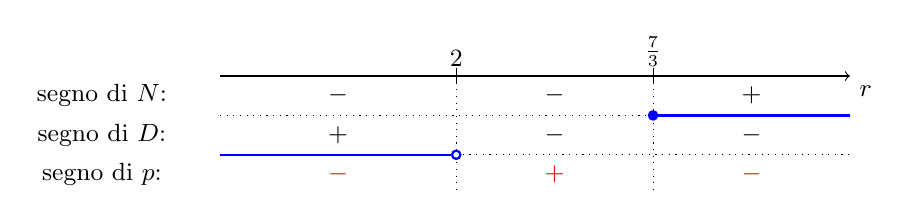
\begin{tikzpicture}[font=\small,x=10mm, y=10mm]

\draw[->] (0,0) -- (8,0) node [below right] () {$r$};

\foreach \x in {3,5.5}{
\draw(\x,3pt)--(\x,-3pt);
\begin{scope}[dotted]
\draw (\x,0) -- (\x,-1.5);
\draw (0,-.5) -- (5.5,-.5);
\draw (3,-1) -- (8,-1);
\end{scope}}

\node[above]  at (3,0) {$2$};
\node[above]  at (5.5,0) {$\frac{7}{3}$};

\begin{scope}[blue,thick]
\draw (5.5,-.5) -- (8,-.5);
\draw (3,-1) -- (0,-1);

\draw[fill=blue] (5.5,-.5)circle (1.5pt);
\draw[fill=white] (3,-1)circle (1.5pt);
\end{scope}

\foreach \x in {-1.5}{
\node  at (\x,-.25) {segno di $N$:};
\node  at (\x,-.75) {segno di $D$:};
\node  at (\x,-1.25) {segno di $p$:};
}
\foreach \z in {1.5,4.25}
\node  at (\z,-.25) {$-$};

\foreach \zi in {4.25,6.75}
\node  at (\zi,-.75) {$-$};

\node  at (6.75,-.25) {$+$};
\node  at (1.5,-.75) {$+$};

\begin{scope}[red]
\foreach \y in {-1.25}{
\foreach \ziv in {4.25}
	\node at (\ziv,\y) {$+$};
\foreach \zv in {1.5,6.75}
\node at (\zv,\y) {$-$};
}
\end{scope}
\end{tikzpicture}
\end{center}
Il sistema è quindi verificato per $1<x\le 3$  cioè: $ \left] 1;~3 \right]$.

% \vspazio\ovalbox{\risolvii \ref{ese:4.75}, \ref{ese:4.76}, \ref{ese:4.77}, 
% \ref{ese:4.78}, \ref{ese:4.79}, \ref{ese:4.80}, \ref{ese:4.81}, 
% \ref{ese:4.82}, 
% \ref{ese:4.83}}
\end{comment}